\documentclass[twoside]{book}

% Packages required by doxygen
\usepackage{fixltx2e}
\usepackage{calc}
\usepackage{doxygen}
\usepackage[export]{adjustbox} % also loads graphicx
\usepackage{graphicx}
\usepackage[utf8]{inputenc}
\usepackage{makeidx}
\usepackage{multicol}
\usepackage{multirow}
\PassOptionsToPackage{warn}{textcomp}
\usepackage{textcomp}
\usepackage[nointegrals]{wasysym}
\usepackage[table]{xcolor}

% Font selection
\usepackage[T1]{fontenc}
\usepackage[scaled=.90]{helvet}
\usepackage{courier}
\usepackage{amssymb}
\usepackage{sectsty}
\renewcommand{\familydefault}{\sfdefault}
\allsectionsfont{%
  \fontseries{bc}\selectfont%
  \color{darkgray}%
}
\renewcommand{\DoxyLabelFont}{%
  \fontseries{bc}\selectfont%
  \color{darkgray}%
}
\newcommand{\+}{\discretionary{\mbox{\scriptsize$\hookleftarrow$}}{}{}}

% Page & text layout
\usepackage{geometry}
\geometry{%
  a4paper,%
  top=2.5cm,%
  bottom=2.5cm,%
  left=2.5cm,%
  right=2.5cm%
}
\tolerance=750
\hfuzz=15pt
\hbadness=750
\setlength{\emergencystretch}{15pt}
\setlength{\parindent}{0cm}
\setlength{\parskip}{3ex plus 2ex minus 2ex}
\makeatletter
\renewcommand{\paragraph}{%
  \@startsection{paragraph}{4}{0ex}{-1.0ex}{1.0ex}{%
    \normalfont\normalsize\bfseries\SS@parafont%
  }%
}
\renewcommand{\subparagraph}{%
  \@startsection{subparagraph}{5}{0ex}{-1.0ex}{1.0ex}{%
    \normalfont\normalsize\bfseries\SS@subparafont%
  }%
}
\makeatother

% Headers & footers
\usepackage{fancyhdr}
\pagestyle{fancyplain}
\fancyhead[LE]{\fancyplain{}{\bfseries\thepage}}
\fancyhead[CE]{\fancyplain{}{}}
\fancyhead[RE]{\fancyplain{}{\bfseries\leftmark}}
\fancyhead[LO]{\fancyplain{}{\bfseries\rightmark}}
\fancyhead[CO]{\fancyplain{}{}}
\fancyhead[RO]{\fancyplain{}{\bfseries\thepage}}
\fancyfoot[LE]{\fancyplain{}{}}
\fancyfoot[CE]{\fancyplain{}{}}
\fancyfoot[RE]{\fancyplain{}{\bfseries\scriptsize Generated by Doxygen }}
\fancyfoot[LO]{\fancyplain{}{\bfseries\scriptsize Generated by Doxygen }}
\fancyfoot[CO]{\fancyplain{}{}}
\fancyfoot[RO]{\fancyplain{}{}}
\renewcommand{\footrulewidth}{0.4pt}
\renewcommand{\chaptermark}[1]{%
  \markboth{#1}{}%
}
\renewcommand{\sectionmark}[1]{%
  \markright{\thesection\ #1}%
}

% Indices & bibliography
\usepackage{natbib}
\usepackage[titles]{tocloft}
\setcounter{tocdepth}{3}
\setcounter{secnumdepth}{5}
\makeindex

% Hyperlinks (required, but should be loaded last)
\usepackage{ifpdf}
\ifpdf
  \usepackage[pdftex,pagebackref=true]{hyperref}
\else
  \usepackage[ps2pdf,pagebackref=true]{hyperref}
\fi
\hypersetup{%
  colorlinks=true,%
  linkcolor=blue,%
  citecolor=blue,%
  unicode%
}

% Custom commands
\newcommand{\clearemptydoublepage}{%
  \newpage{\pagestyle{empty}\cleardoublepage}%
}

\usepackage{caption}
\captionsetup{labelsep=space,justification=centering,font={bf},singlelinecheck=off,skip=4pt,position=top}

%===== C O N T E N T S =====

\begin{document}

% Titlepage & ToC
\hypersetup{pageanchor=false,
             bookmarksnumbered=true,
             pdfencoding=unicode
            }
\pagenumbering{alph}
\begin{titlepage}
\vspace*{7cm}
\begin{center}%
{\Large Computational Methods }\\
\vspace*{1cm}
{\large Generated by Doxygen 1.8.13}\\
\end{center}
\end{titlepage}
\clearemptydoublepage
\pagenumbering{roman}
\tableofcontents
\clearemptydoublepage
\pagenumbering{arabic}
\hypersetup{pageanchor=true}

%--- Begin generated contents ---
\chapter{Hierarchical Index}
\section{Class Hierarchy}
This inheritance list is sorted roughly, but not completely, alphabetically\+:\begin{DoxyCompactList}
\item \contentsline{section}{Output}{\pageref{class_output}}{}
\item \contentsline{section}{Solution}{\pageref{class_solution}}{}
\begin{DoxyCompactList}
\item \contentsline{section}{Analytical\+Solution}{\pageref{class_analytical_solution}}{}
\item \contentsline{section}{Crank\+Nicholson\+Method}{\pageref{class_crank_nicholson_method}}{}
\item \contentsline{section}{Du\+Fort\+Frankel\+Method}{\pageref{class_du_fort_frankel_method}}{}
\item \contentsline{section}{Laasonen\+Method}{\pageref{class_laasonen_method}}{}
\item \contentsline{section}{Richardson\+Method}{\pageref{class_richardson_method}}{}
\end{DoxyCompactList}
\item \contentsline{section}{Tools}{\pageref{class_tools}}{}
\end{DoxyCompactList}

\chapter{Class Index}
\section{Class List}
Here are the classes, structs, unions and interfaces with brief descriptions\+:\begin{DoxyCompactList}
\item\contentsline{section}{\hyperlink{class_matrix}{Matrix} }{\pageref{class_matrix}}{}
\item\contentsline{section}{\hyperlink{class_solution}{Solution} }{\pageref{class_solution}}{}
\item\contentsline{section}{\hyperlink{class_vector}{Vector} }{\pageref{class_vector}}{}
\end{DoxyCompactList}

\chapter{Class Documentation}
\hypertarget{class_analytical_solution}{}\section{Analytical\+Solution Class Reference}
\label{class_analytical_solution}\index{Analytical\+Solution@{Analytical\+Solution}}
Inheritance diagram for Analytical\+Solution\+:\begin{figure}[H]
\begin{center}
\leavevmode
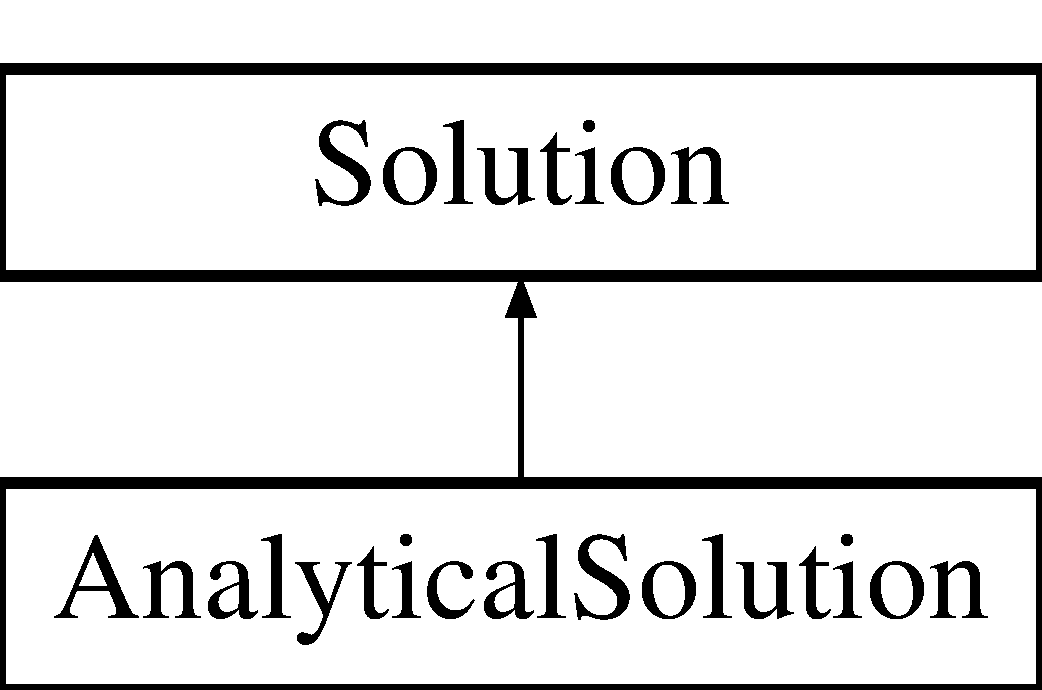
\includegraphics[height=2.000000cm]{class_analytical_solution}
\end{center}
\end{figure}
\subsection*{Public Member Functions}
\begin{DoxyCompactItemize}
\item 
\mbox{\Hypertarget{class_analytical_solution_a9522a4a13b61dcc7f145e0fb39e5016d}\label{class_analytical_solution_a9522a4a13b61dcc7f145e0fb39e5016d}} 
{\bfseries Analytical\+Solution} (std\+::vector$<$ double $>$ v)
\item 
\mbox{\Hypertarget{class_analytical_solution_ae1ebc556a8dfed55b6c463625545d919}\label{class_analytical_solution_ae1ebc556a8dfed55b6c463625545d919}} 
void {\bfseries compute} ()
\end{DoxyCompactItemize}
\subsection*{Protected Attributes}
\begin{DoxyCompactItemize}
\item 
\mbox{\Hypertarget{class_analytical_solution_a7790fe079a6319530e2d203c5ff64b23}\label{class_analytical_solution_a7790fe079a6319530e2d203c5ff64b23}} 
const double {\bfseries PI} = 3.\+141592
\end{DoxyCompactItemize}


The documentation for this class was generated from the following files\+:\begin{DoxyCompactItemize}
\item 
Analytical\+Solution.\+h\item 
Analytical\+Solution.\+cpp\end{DoxyCompactItemize}

\hypertarget{class_crank_nicholson_method}{}\section{Crank\+Nicholson\+Method Class Reference}
\label{class_crank_nicholson_method}\index{Crank\+Nicholson\+Method@{Crank\+Nicholson\+Method}}
Inheritance diagram for Crank\+Nicholson\+Method\+:\begin{figure}[H]
\begin{center}
\leavevmode
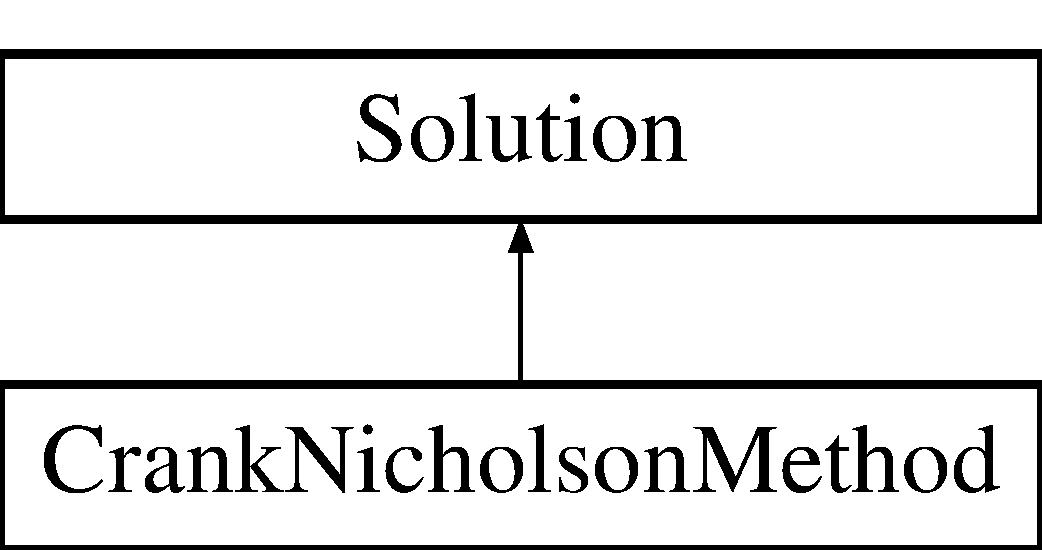
\includegraphics[height=2.000000cm]{class_crank_nicholson_method}
\end{center}
\end{figure}
\subsection*{Public Member Functions}
\begin{DoxyCompactItemize}
\item 
\hyperlink{class_crank_nicholson_method_ae5052444cd3f042a554bb74d9ac556e0}{Crank\+Nicholson\+Method} ()
\item 
\hyperlink{class_crank_nicholson_method_a9738c40cac3d4f37775d6211544b178f}{Crank\+Nicholson\+Method} (std\+::vector$<$ std\+::vector$<$ double $>$$>$ sols)
\item 
void \hyperlink{class_crank_nicholson_method_a10558e5238673e11a76b4e10e8c588b4}{compute} ()
\end{DoxyCompactItemize}
\subsection*{Additional Inherited Members}


\subsection{Constructor \& Destructor Documentation}
\mbox{\Hypertarget{class_crank_nicholson_method_ae5052444cd3f042a554bb74d9ac556e0}\label{class_crank_nicholson_method_ae5052444cd3f042a554bb74d9ac556e0}} 
\index{Crank\+Nicholson\+Method@{Crank\+Nicholson\+Method}!Crank\+Nicholson\+Method@{Crank\+Nicholson\+Method}}
\index{Crank\+Nicholson\+Method@{Crank\+Nicholson\+Method}!Crank\+Nicholson\+Method@{Crank\+Nicholson\+Method}}
\subsubsection{\texorpdfstring{Crank\+Nicholson\+Method()}{CrankNicholsonMethod()}\hspace{0.1cm}{\footnotesize\ttfamily [1/2]}}
{\footnotesize\ttfamily Crank\+Nicholson\+Method\+::\+Crank\+Nicholson\+Method (\begin{DoxyParamCaption}{ }\end{DoxyParamCaption})}

Creates an empty \hyperlink{class_crank_nicholson_method}{Crank\+Nicholson\+Method} object \begin{DoxySeeAlso}{See also}
\hyperlink{class_crank_nicholson_method}{Crank\+Nicholson\+Method(\+Vector$<$\+Vector$<$double$>$$>$ sols)}; 
\end{DoxySeeAlso}
\mbox{\Hypertarget{class_crank_nicholson_method_a9738c40cac3d4f37775d6211544b178f}\label{class_crank_nicholson_method_a9738c40cac3d4f37775d6211544b178f}} 
\index{Crank\+Nicholson\+Method@{Crank\+Nicholson\+Method}!Crank\+Nicholson\+Method@{Crank\+Nicholson\+Method}}
\index{Crank\+Nicholson\+Method@{Crank\+Nicholson\+Method}!Crank\+Nicholson\+Method@{Crank\+Nicholson\+Method}}
\subsubsection{\texorpdfstring{Crank\+Nicholson\+Method()}{CrankNicholsonMethod()}\hspace{0.1cm}{\footnotesize\ttfamily [2/2]}}
{\footnotesize\ttfamily Crank\+Nicholson\+Method\+::\+Crank\+Nicholson\+Method (\begin{DoxyParamCaption}\item[{std\+::vector$<$ std\+::vector$<$ double $>$$>$}]{sols }\end{DoxyParamCaption})}

Creates an \hyperlink{class_crank_nicholson_method}{Crank\+Nicholson\+Method} object from a vector of double vectors. \begin{DoxySeeAlso}{See also}
\hyperlink{class_crank_nicholson_method_ae5052444cd3f042a554bb74d9ac556e0}{Crank\+Nicholson\+Method()}; 
\end{DoxySeeAlso}

\begin{DoxyParams}{Parameters}
{\em sols} & \hyperlink{class_vector}{Vector} of double vectors that the new \hyperlink{class_solution}{Solution} will use. \\
\hline
\end{DoxyParams}

\begin{DoxyParams}{Parameters}
{\em sols} & std\+::vector$<$std\+::vector$<$double$>$$>$. \hyperlink{class_vector}{Vector} of double vectors that the new \hyperlink{class_solution}{Solution} will use. \\
\hline
\end{DoxyParams}


\subsection{Member Function Documentation}
\mbox{\Hypertarget{class_crank_nicholson_method_a10558e5238673e11a76b4e10e8c588b4}\label{class_crank_nicholson_method_a10558e5238673e11a76b4e10e8c588b4}} 
\index{Crank\+Nicholson\+Method@{Crank\+Nicholson\+Method}!compute@{compute}}
\index{compute@{compute}!Crank\+Nicholson\+Method@{Crank\+Nicholson\+Method}}
\subsubsection{\texorpdfstring{compute()}{compute()}}
{\footnotesize\ttfamily void Crank\+Nicholson\+Method\+::compute (\begin{DoxyParamCaption}{ }\end{DoxyParamCaption})}

Computes and stores the values for the \hyperlink{class_solution}{Solution} using this method. 

The documentation for this class was generated from the following files\+:\begin{DoxyCompactItemize}
\item 
Crank\+Nicholson\+Method.\+h\item 
Crank\+Nicholson\+Method.\+cpp\end{DoxyCompactItemize}

\hypertarget{class_du_fort_frankel_method}{}\section{Du\+Fort\+Frankel\+Method Class Reference}
\label{class_du_fort_frankel_method}\index{Du\+Fort\+Frankel\+Method@{Du\+Fort\+Frankel\+Method}}


{\ttfamily \#include $<$Du\+Fort\+Frankel\+Method.\+h$>$}

Inheritance diagram for Du\+Fort\+Frankel\+Method\+:\begin{figure}[H]
\begin{center}
\leavevmode
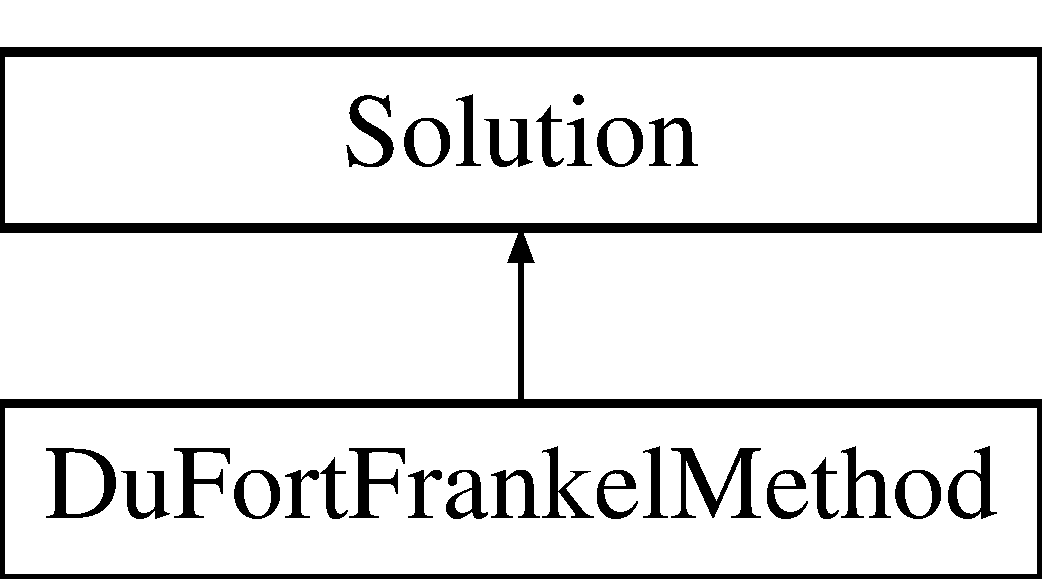
\includegraphics[height=2.000000cm]{class_du_fort_frankel_method}
\end{center}
\end{figure}
\subsection*{Public Member Functions}
\begin{DoxyCompactItemize}
\item 
\hyperlink{class_du_fort_frankel_method_ae4f8e7c2d498265fa8b8e6ea0bd74288}{Du\+Fort\+Frankel\+Method} ()
\item 
\hyperlink{class_du_fort_frankel_method_a5914f09f3f3aa00d0ac1d270e73613e2}{Du\+Fort\+Frankel\+Method} (std\+::vector$<$ std\+::vector$<$ double $>$$>$ sols)
\item 
void \hyperlink{class_du_fort_frankel_method_a68b9ad88883a71daba4c2fc92355b173}{compute} ()
\end{DoxyCompactItemize}
\subsection*{Additional Inherited Members}


\subsection{Detailed Description}
The \hyperlink{class_du_fort_frankel_method}{Du\+Fort\+Frankel\+Method} is an explicit and unconditionally stable method. ~\newline
 This method is a variation of the \hyperlink{class_richardson_method}{Richardson\+Method}. 

\subsection{Constructor \& Destructor Documentation}
\mbox{\Hypertarget{class_du_fort_frankel_method_ae4f8e7c2d498265fa8b8e6ea0bd74288}\label{class_du_fort_frankel_method_ae4f8e7c2d498265fa8b8e6ea0bd74288}} 
\index{Du\+Fort\+Frankel\+Method@{Du\+Fort\+Frankel\+Method}!Du\+Fort\+Frankel\+Method@{Du\+Fort\+Frankel\+Method}}
\index{Du\+Fort\+Frankel\+Method@{Du\+Fort\+Frankel\+Method}!Du\+Fort\+Frankel\+Method@{Du\+Fort\+Frankel\+Method}}
\subsubsection{\texorpdfstring{Du\+Fort\+Frankel\+Method()}{DuFortFrankelMethod()}\hspace{0.1cm}{\footnotesize\ttfamily [1/2]}}
{\footnotesize\ttfamily Du\+Fort\+Frankel\+Method\+::\+Du\+Fort\+Frankel\+Method (\begin{DoxyParamCaption}{ }\end{DoxyParamCaption})}

Creates an empty \hyperlink{class_du_fort_frankel_method}{Du\+Fort\+Frankel\+Method} object \begin{DoxySeeAlso}{See also}
\hyperlink{class_du_fort_frankel_method}{Du\+Fort\+Frankel\+Method(\+Vector$<$\+Vector$<$double$>$$>$ sols)}; 
\end{DoxySeeAlso}
\mbox{\Hypertarget{class_du_fort_frankel_method_a5914f09f3f3aa00d0ac1d270e73613e2}\label{class_du_fort_frankel_method_a5914f09f3f3aa00d0ac1d270e73613e2}} 
\index{Du\+Fort\+Frankel\+Method@{Du\+Fort\+Frankel\+Method}!Du\+Fort\+Frankel\+Method@{Du\+Fort\+Frankel\+Method}}
\index{Du\+Fort\+Frankel\+Method@{Du\+Fort\+Frankel\+Method}!Du\+Fort\+Frankel\+Method@{Du\+Fort\+Frankel\+Method}}
\subsubsection{\texorpdfstring{Du\+Fort\+Frankel\+Method()}{DuFortFrankelMethod()}\hspace{0.1cm}{\footnotesize\ttfamily [2/2]}}
{\footnotesize\ttfamily Du\+Fort\+Frankel\+Method\+::\+Du\+Fort\+Frankel\+Method (\begin{DoxyParamCaption}\item[{std\+::vector$<$ std\+::vector$<$ double $>$$>$}]{sols }\end{DoxyParamCaption})}

Creates an \hyperlink{class_du_fort_frankel_method}{Du\+Fort\+Frankel\+Method} object from a vector of double vectors. \begin{DoxySeeAlso}{See also}
\hyperlink{class_du_fort_frankel_method_ae4f8e7c2d498265fa8b8e6ea0bd74288}{Du\+Fort\+Frankel\+Method()}; 
\end{DoxySeeAlso}

\begin{DoxyParams}{Parameters}
{\em sols} & \hyperlink{class_vector}{Vector} of double vectors that the new \hyperlink{class_solution}{Solution} will use. \\
\hline
\end{DoxyParams}

\begin{DoxyParams}{Parameters}
{\em sols} & std\+::vector$<$std\+::vector$<$double$>$$>$. \hyperlink{class_vector}{Vector} of double vectors that the new \hyperlink{class_solution}{Solution} will use. \\
\hline
\end{DoxyParams}


\subsection{Member Function Documentation}
\mbox{\Hypertarget{class_du_fort_frankel_method_a68b9ad88883a71daba4c2fc92355b173}\label{class_du_fort_frankel_method_a68b9ad88883a71daba4c2fc92355b173}} 
\index{Du\+Fort\+Frankel\+Method@{Du\+Fort\+Frankel\+Method}!compute@{compute}}
\index{compute@{compute}!Du\+Fort\+Frankel\+Method@{Du\+Fort\+Frankel\+Method}}
\subsubsection{\texorpdfstring{compute()}{compute()}}
{\footnotesize\ttfamily void Du\+Fort\+Frankel\+Method\+::compute (\begin{DoxyParamCaption}{ }\end{DoxyParamCaption})}

Computes and stores the values for the \hyperlink{class_solution}{Solution} using this method.

Computes and stores the values for the \hyperlink{class_solution}{Solution} using the Du Fort Frankel method as well as the forward time, central space method for certain timestep. 

The documentation for this class was generated from the following files\+:\begin{DoxyCompactItemize}
\item 
Du\+Fort\+Frankel\+Method.\+h\item 
Du\+Fort\+Frankel\+Method.\+cpp\end{DoxyCompactItemize}

\hypertarget{class_laasonen_method}{}\section{Laasonen\+Method Class Reference}
\label{class_laasonen_method}\index{Laasonen\+Method@{Laasonen\+Method}}
Inheritance diagram for Laasonen\+Method\+:\begin{figure}[H]
\begin{center}
\leavevmode
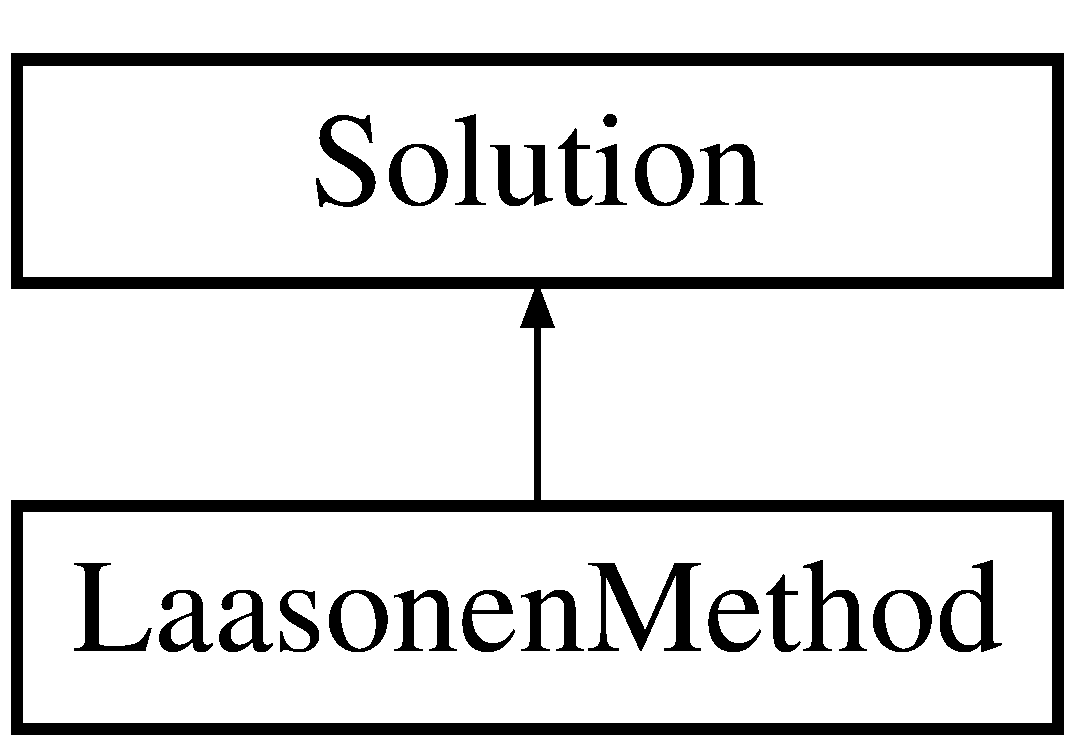
\includegraphics[height=2.000000cm]{class_laasonen_method}
\end{center}
\end{figure}
\subsection*{Public Member Functions}
\begin{DoxyCompactItemize}
\item 
\mbox{\Hypertarget{class_laasonen_method_a82f953953a8425ad936f75ddc9954a34}\label{class_laasonen_method_a82f953953a8425ad936f75ddc9954a34}} 
{\bfseries Laasonen\+Method} (std\+::vector$<$ double $>$ v)
\item 
\mbox{\Hypertarget{class_laasonen_method_a8eb364e47a161f8ca4700c8899786910}\label{class_laasonen_method_a8eb364e47a161f8ca4700c8899786910}} 
void {\bfseries add\+ToL} (std\+::vector$<$ double $>$ row)
\item 
\mbox{\Hypertarget{class_laasonen_method_a00aa549123730dc16651d06db8377523}\label{class_laasonen_method_a00aa549123730dc16651d06db8377523}} 
std\+::vector$<$ std\+::vector$<$ double $>$ $>$ {\bfseries getL} ()
\item 
void \hyperlink{class_laasonen_method_ac5507d58a6c59f0ba9eaa3ca54a51f5d}{compute} ()
\end{DoxyCompactItemize}
\subsection*{Protected Attributes}
\begin{DoxyCompactItemize}
\item 
\mbox{\Hypertarget{class_laasonen_method_a9261b579f612bf4ce6b0d85cbe39bb56}\label{class_laasonen_method_a9261b579f612bf4ce6b0d85cbe39bb56}} 
double {\bfseries C} = (\hyperlink{class_solution_a116a08a1a8793618fb5269016cfd9b61}{deltaT}$\ast$\hyperlink{class_solution_af647b9b893549259060034672babb0f8}{D}) / pow(\hyperlink{class_solution_a8e97e5534ddcde31983432b8fb2050ff}{deltaX}, 2)
\item 
\mbox{\Hypertarget{class_laasonen_method_a9bfc5f53066a6dec716d07d046274669}\label{class_laasonen_method_a9bfc5f53066a6dec716d07d046274669}} 
int {\bfseries posL} = 0
\item 
\mbox{\Hypertarget{class_laasonen_method_addfca3dd9aebb1fc71ad049f11a12480}\label{class_laasonen_method_addfca3dd9aebb1fc71ad049f11a12480}} 
std\+::vector$<$ std\+::vector$<$ double $>$ $>$ {\bfseries L}
\end{DoxyCompactItemize}


\subsection{Member Function Documentation}
\mbox{\Hypertarget{class_laasonen_method_ac5507d58a6c59f0ba9eaa3ca54a51f5d}\label{class_laasonen_method_ac5507d58a6c59f0ba9eaa3ca54a51f5d}} 
\index{Laasonen\+Method@{Laasonen\+Method}!compute@{compute}}
\index{compute@{compute}!Laasonen\+Method@{Laasonen\+Method}}
\subsubsection{\texorpdfstring{compute()}{compute()}}
{\footnotesize\ttfamily void Laasonen\+Method\+::compute (\begin{DoxyParamCaption}{ }\end{DoxyParamCaption})}

Computes and stores the values for the \hyperlink{class_solution}{Solution} using this method. 

The documentation for this class was generated from the following files\+:\begin{DoxyCompactItemize}
\item 
Laasonen\+Method.\+h\item 
Laasonen\+Method.\+cpp\end{DoxyCompactItemize}

\hypertarget{class_output}{}\section{Output Class Reference}
\label{class_output}\index{Output@{Output}}


{\ttfamily \#include $<$Output.\+h$>$}

\subsection*{Static Public Member Functions}
\begin{DoxyCompactItemize}
\item 
static void \hyperlink{class_output_a79b3b86314e979457e5aac1ff4840605}{print\+Solution} (std\+::vector$<$ std\+::vector$<$ double $>$$>$ sols)
\item 
\mbox{\Hypertarget{class_output_a0d39b68ef723d6372f7c17e967a1d29a}\label{class_output_a0d39b68ef723d6372f7c17e967a1d29a}} 
static void {\bfseries export\+Solution} (\hyperlink{class_solution}{Solution} obj, double x\+Size, std\+::string name)
\end{DoxyCompactItemize}


\subsection{Detailed Description}
The \hyperlink{class_output}{Output} class is utilised to export the content ~\newline
 of the solutions as files or simply show the ~\newline
 results on the console. 

\subsection{Member Function Documentation}
\mbox{\Hypertarget{class_output_a79b3b86314e979457e5aac1ff4840605}\label{class_output_a79b3b86314e979457e5aac1ff4840605}} 
\index{Output@{Output}!print\+Solution@{print\+Solution}}
\index{print\+Solution@{print\+Solution}!Output@{Output}}
\subsubsection{\texorpdfstring{print\+Solution()}{printSolution()}}
{\footnotesize\ttfamily void Output\+::print\+Solution (\begin{DoxyParamCaption}\item[{std\+::vector$<$ std\+::vector$<$ double $>$$>$}]{v }\end{DoxyParamCaption})\hspace{0.3cm}{\ttfamily [static]}}

Prints on console all the solutions stored in a \hyperlink{class_solution}{Solution} object. 
\begin{DoxyParams}{Parameters}
{\em sols} & This should be the all\+Solutions attribute from the \hyperlink{class_solution}{Solution} object we want to print.\\
\hline
\end{DoxyParams}
Print all solutions from a vector of double vectors. 
\begin{DoxyParams}{Parameters}
{\em v} & std\+::vector$<$std\+::vector$<$double$>$$>$. \hyperlink{class_vector}{Vector} of double vectors that we want to print. \\
\hline
\end{DoxyParams}


The documentation for this class was generated from the following files\+:\begin{DoxyCompactItemize}
\item 
Output.\+h\item 
Output.\+cpp\end{DoxyCompactItemize}

\hypertarget{class_richardson_method}{}\section{Richardson\+Method Class Reference}
\label{class_richardson_method}\index{Richardson\+Method@{Richardson\+Method}}


{\ttfamily \#include $<$Richardson\+Method.\+h$>$}

Inheritance diagram for Richardson\+Method\+:\begin{figure}[H]
\begin{center}
\leavevmode
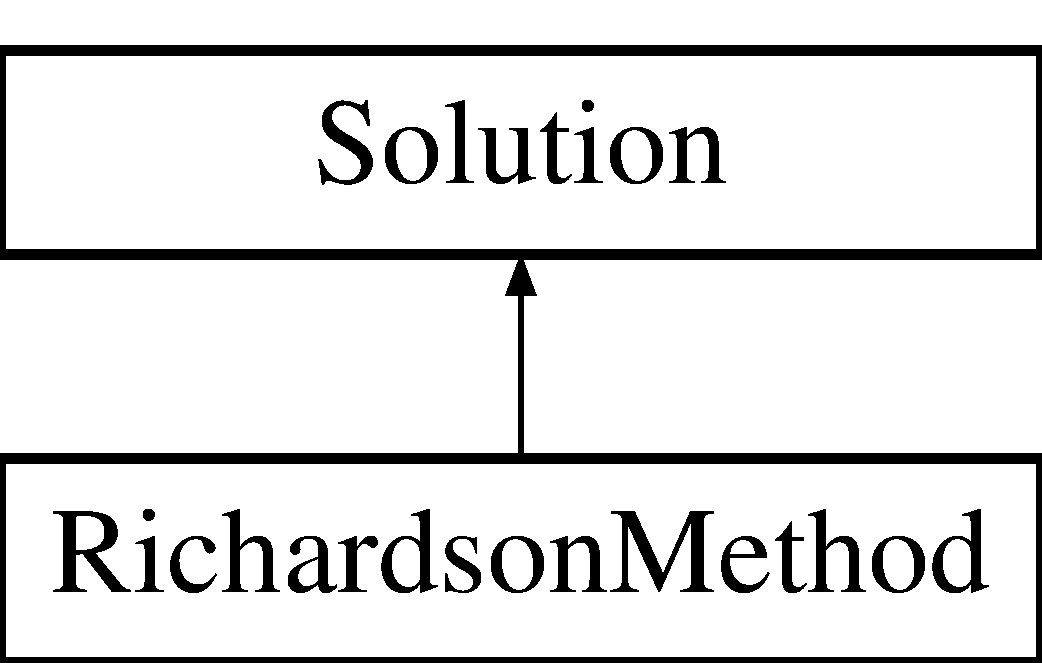
\includegraphics[height=2.000000cm]{class_richardson_method}
\end{center}
\end{figure}
\subsection*{Public Member Functions}
\begin{DoxyCompactItemize}
\item 
\hyperlink{class_richardson_method_a01c839ad5a09cd0e0a9e56ad8e43f980}{Richardson\+Method} ()
\item 
\hyperlink{class_richardson_method_a11cf699f84bdd051e16983096c6d4979}{Richardson\+Method} (std\+::vector$<$ std\+::vector$<$ double $>$$>$ sols)
\item 
void \hyperlink{class_richardson_method_acefe085864b041381f1a7fd3af46d7fb}{compute} ()
\end{DoxyCompactItemize}
\subsection*{Additional Inherited Members}


\subsection{Detailed Description}
The \hyperlink{class_richardson_method}{Richardson\+Method} is an explicit and unconditionally unstable method. ~\newline
 This method will produce a solution with an error increasing in time. 

\subsection{Constructor \& Destructor Documentation}
\mbox{\Hypertarget{class_richardson_method_a01c839ad5a09cd0e0a9e56ad8e43f980}\label{class_richardson_method_a01c839ad5a09cd0e0a9e56ad8e43f980}} 
\index{Richardson\+Method@{Richardson\+Method}!Richardson\+Method@{Richardson\+Method}}
\index{Richardson\+Method@{Richardson\+Method}!Richardson\+Method@{Richardson\+Method}}
\subsubsection{\texorpdfstring{Richardson\+Method()}{RichardsonMethod()}\hspace{0.1cm}{\footnotesize\ttfamily [1/2]}}
{\footnotesize\ttfamily Richardson\+Method\+::\+Richardson\+Method (\begin{DoxyParamCaption}{ }\end{DoxyParamCaption})}

Creates an empty \hyperlink{class_richardson_method}{Richardson\+Method} object \begin{DoxySeeAlso}{See also}
\hyperlink{class_richardson_method}{Richardson\+Method(\+Vector$<$\+Vector$<$double$>$$>$ sols)}; 
\end{DoxySeeAlso}
\mbox{\Hypertarget{class_richardson_method_a11cf699f84bdd051e16983096c6d4979}\label{class_richardson_method_a11cf699f84bdd051e16983096c6d4979}} 
\index{Richardson\+Method@{Richardson\+Method}!Richardson\+Method@{Richardson\+Method}}
\index{Richardson\+Method@{Richardson\+Method}!Richardson\+Method@{Richardson\+Method}}
\subsubsection{\texorpdfstring{Richardson\+Method()}{RichardsonMethod()}\hspace{0.1cm}{\footnotesize\ttfamily [2/2]}}
{\footnotesize\ttfamily Richardson\+Method\+::\+Richardson\+Method (\begin{DoxyParamCaption}\item[{std\+::vector$<$ std\+::vector$<$ double $>$$>$}]{sols }\end{DoxyParamCaption})}

Creates an \hyperlink{class_richardson_method}{Richardson\+Method} object from a vector of double vectors. \begin{DoxySeeAlso}{See also}
\hyperlink{class_richardson_method_a01c839ad5a09cd0e0a9e56ad8e43f980}{Richardson\+Method()}; 
\end{DoxySeeAlso}

\begin{DoxyParams}{Parameters}
{\em sols} & Vector of double vectors that the new \hyperlink{class_solution}{Solution} will use. \\
\hline
\end{DoxyParams}

\begin{DoxyParams}{Parameters}
{\em sols} & std\+::vector$<$std\+::vector$<$double$>$$>$. Vector of double vectors that the new \hyperlink{class_solution}{Solution} will use. \\
\hline
\end{DoxyParams}


\subsection{Member Function Documentation}
\mbox{\Hypertarget{class_richardson_method_acefe085864b041381f1a7fd3af46d7fb}\label{class_richardson_method_acefe085864b041381f1a7fd3af46d7fb}} 
\index{Richardson\+Method@{Richardson\+Method}!compute@{compute}}
\index{compute@{compute}!Richardson\+Method@{Richardson\+Method}}
\subsubsection{\texorpdfstring{compute()}{compute()}}
{\footnotesize\ttfamily void Richardson\+Method\+::compute (\begin{DoxyParamCaption}{ }\end{DoxyParamCaption})}

Computes and stores the values for the \hyperlink{class_solution}{Solution} using this method.

Computes and stores the values for the \hyperlink{class_solution}{Solution} using the Richardson method as well as the forward time, central space method for certain timestep. 

The documentation for this class was generated from the following files\+:\begin{DoxyCompactItemize}
\item 
Richardson\+Method.\+h\item 
Richardson\+Method.\+cpp\end{DoxyCompactItemize}

\hypertarget{class_solution}{}\section{Solution Class Reference}
\label{class_solution}\index{Solution@{Solution}}
Inheritance diagram for Solution\+:\begin{figure}[H]
\begin{center}
\leavevmode
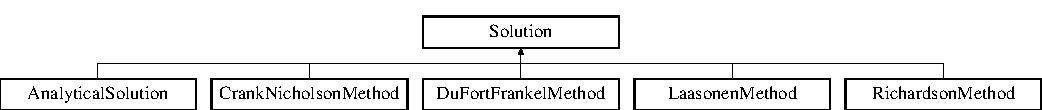
\includegraphics[height=2.000000cm]{class_solution}
\end{center}
\end{figure}
\subsection*{Public Member Functions}
\begin{DoxyCompactItemize}
\item 
\hyperlink{class_solution_ab55bd4b023d596ce11aaf737b9a6123b}{Solution} ()
\item 
\hyperlink{class_solution_a3a2983c7a229e6d7408471b4dc48fe61}{Solution} (std\+::vector$<$ double $>$ v)
\item 
std\+::vector$<$ std\+::vector$<$ double $>$ $>$ \hyperlink{class_solution_abd28abd062adb793866fd5e1c8ef8639}{get\+All\+Solutions} ()
\item 
std\+::vector$<$ double $>$ \hyperlink{class_solution_ae92d4a6070f6e5879698754fa5547ee3}{get\+Current\+Solution} ()
\item 
void \hyperlink{class_solution_a0ea58d9480ccb4e344c377f4861e1e7f}{add\+To\+All\+Solutions} (std\+::vector$<$ double $>$ v)
\item 
void \hyperlink{class_solution_a32dad1b34b687cb439a2a60881e50402}{set\+Current\+Solution} (std\+::vector$<$ double $>$ v)
\end{DoxyCompactItemize}
\subsection*{Protected Attributes}
\begin{DoxyCompactItemize}
\item 
\mbox{\Hypertarget{class_solution_a8e97e5534ddcde31983432b8fb2050ff}\label{class_solution_a8e97e5534ddcde31983432b8fb2050ff}} 
double \hyperlink{class_solution_a8e97e5534ddcde31983432b8fb2050ff}{deltaX} = 0.\+05
\begin{DoxyCompactList}\small\item\em can be changed for different problems. \end{DoxyCompactList}\item 
\mbox{\Hypertarget{class_solution_a116a08a1a8793618fb5269016cfd9b61}\label{class_solution_a116a08a1a8793618fb5269016cfd9b61}} 
double \hyperlink{class_solution_a116a08a1a8793618fb5269016cfd9b61}{deltaT} = 0.\+01
\begin{DoxyCompactList}\small\item\em can be changed for different problems. \end{DoxyCompactList}\item 
\mbox{\Hypertarget{class_solution_af647b9b893549259060034672babb0f8}\label{class_solution_af647b9b893549259060034672babb0f8}} 
double \hyperlink{class_solution_af647b9b893549259060034672babb0f8}{D} = 0.\+1
\begin{DoxyCompactList}\small\item\em Diffusivity of the material in the problem. \end{DoxyCompactList}\item 
\mbox{\Hypertarget{class_solution_afa80e5854fb5af93932f445e426c7f66}\label{class_solution_afa80e5854fb5af93932f445e426c7f66}} 
double \hyperlink{class_solution_afa80e5854fb5af93932f445e426c7f66}{L} = 1.\+0
\begin{DoxyCompactList}\small\item\em Length of the problem. \end{DoxyCompactList}\item 
\mbox{\Hypertarget{class_solution_aca95282163f453b465bb1991c596a34e}\label{class_solution_aca95282163f453b465bb1991c596a34e}} 
int \hyperlink{class_solution_aca95282163f453b465bb1991c596a34e}{n} = 20
\begin{DoxyCompactList}\small\item\em The size of the solution should be\+: L / deltaX. \end{DoxyCompactList}\item 
\mbox{\Hypertarget{class_solution_a09fa8d2538a87e8d9cba2ee682f729ac}\label{class_solution_a09fa8d2538a87e8d9cba2ee682f729ac}} 
std\+::vector$<$ std\+::vector$<$ double $>$ $>$ \hyperlink{class_solution_a09fa8d2538a87e8d9cba2ee682f729ac}{all\+Solutions}
\begin{DoxyCompactList}\small\item\em We collect in a vector of vectors all solutions we think will be relevant. \end{DoxyCompactList}\item 
\mbox{\Hypertarget{class_solution_af933662f6d08824b37f315fc36678c3b}\label{class_solution_af933662f6d08824b37f315fc36678c3b}} 
int \hyperlink{class_solution_af933662f6d08824b37f315fc36678c3b}{all\+Sol\+Pos} = 0
\begin{DoxyCompactList}\small\item\em We control the number of elements inside the all\+Solutions vector. \end{DoxyCompactList}\item 
\mbox{\Hypertarget{class_solution_ae15c62e099b4ad8a337b62fd05283cd8}\label{class_solution_ae15c62e099b4ad8a337b62fd05283cd8}} 
std\+::vector$<$ double $>$ \hyperlink{class_solution_ae15c62e099b4ad8a337b62fd05283cd8}{solution}
\begin{DoxyCompactList}\small\item\em \hyperlink{class_vector}{Vector} with the solution for a certain timestep. \end{DoxyCompactList}\end{DoxyCompactItemize}


\subsection{Constructor \& Destructor Documentation}
\mbox{\Hypertarget{class_solution_ab55bd4b023d596ce11aaf737b9a6123b}\label{class_solution_ab55bd4b023d596ce11aaf737b9a6123b}} 
\index{Solution@{Solution}!Solution@{Solution}}
\index{Solution@{Solution}!Solution@{Solution}}
\subsubsection{\texorpdfstring{Solution()}{Solution()}\hspace{0.1cm}{\footnotesize\ttfamily [1/2]}}
{\footnotesize\ttfamily Solution\+::\+Solution (\begin{DoxyParamCaption}{ }\end{DoxyParamCaption})}

Creates an empty \hyperlink{class_solution}{Solution} object \begin{DoxySeeAlso}{See also}
\hyperlink{class_solution}{Solution(\+Vector v)}; 
\end{DoxySeeAlso}
\mbox{\Hypertarget{class_solution_a3a2983c7a229e6d7408471b4dc48fe61}\label{class_solution_a3a2983c7a229e6d7408471b4dc48fe61}} 
\index{Solution@{Solution}!Solution@{Solution}}
\index{Solution@{Solution}!Solution@{Solution}}
\subsubsection{\texorpdfstring{Solution()}{Solution()}\hspace{0.1cm}{\footnotesize\ttfamily [2/2]}}
{\footnotesize\ttfamily Solution\+::\+Solution (\begin{DoxyParamCaption}\item[{std\+::vector$<$ double $>$}]{v }\end{DoxyParamCaption})}

creates a \hyperlink{class_solution}{Solution} object from an array. \begin{DoxySeeAlso}{See also}
\hyperlink{class_solution_ab55bd4b023d596ce11aaf737b9a6123b}{Solution()}; 
\end{DoxySeeAlso}

\begin{DoxyParams}{Parameters}
{\em v} & \hyperlink{class_vector}{Vector} taken as solution \\
\hline
\end{DoxyParams}

\begin{DoxyParams}{Parameters}
{\em v} & std\+::vector$<$double$>$. vector taken as solution \\
\hline
\end{DoxyParams}


\subsection{Member Function Documentation}
\mbox{\Hypertarget{class_solution_a0ea58d9480ccb4e344c377f4861e1e7f}\label{class_solution_a0ea58d9480ccb4e344c377f4861e1e7f}} 
\index{Solution@{Solution}!add\+To\+All\+Solutions@{add\+To\+All\+Solutions}}
\index{add\+To\+All\+Solutions@{add\+To\+All\+Solutions}!Solution@{Solution}}
\subsubsection{\texorpdfstring{add\+To\+All\+Solutions()}{addToAllSolutions()}}
{\footnotesize\ttfamily void Solution\+::add\+To\+All\+Solutions (\begin{DoxyParamCaption}\item[{std\+::vector$<$ double $>$}]{v }\end{DoxyParamCaption})}

changes all\+Solutions \begin{DoxySeeAlso}{See also}
\hyperlink{class_solution_a32dad1b34b687cb439a2a60881e50402}{set\+Current\+Solution()} 
\end{DoxySeeAlso}
\mbox{\Hypertarget{class_solution_abd28abd062adb793866fd5e1c8ef8639}\label{class_solution_abd28abd062adb793866fd5e1c8ef8639}} 
\index{Solution@{Solution}!get\+All\+Solutions@{get\+All\+Solutions}}
\index{get\+All\+Solutions@{get\+All\+Solutions}!Solution@{Solution}}
\subsubsection{\texorpdfstring{get\+All\+Solutions()}{getAllSolutions()}}
{\footnotesize\ttfamily std\+::vector$<$ std\+::vector$<$ double $>$ $>$ Solution\+::get\+All\+Solutions (\begin{DoxyParamCaption}{ }\end{DoxyParamCaption})}

Returns all solutions stored in the \hyperlink{class_solution}{Solution} object. \begin{DoxySeeAlso}{See also}
\hyperlink{class_solution_ae92d4a6070f6e5879698754fa5547ee3}{get\+Current\+Solution()} 
\end{DoxySeeAlso}
\mbox{\Hypertarget{class_solution_ae92d4a6070f6e5879698754fa5547ee3}\label{class_solution_ae92d4a6070f6e5879698754fa5547ee3}} 
\index{Solution@{Solution}!get\+Current\+Solution@{get\+Current\+Solution}}
\index{get\+Current\+Solution@{get\+Current\+Solution}!Solution@{Solution}}
\subsubsection{\texorpdfstring{get\+Current\+Solution()}{getCurrentSolution()}}
{\footnotesize\ttfamily std\+::vector$<$ double $>$ Solution\+::get\+Current\+Solution (\begin{DoxyParamCaption}{ }\end{DoxyParamCaption})}

Returns current solution stored in the object. \begin{DoxySeeAlso}{See also}
\hyperlink{class_solution_abd28abd062adb793866fd5e1c8ef8639}{get\+All\+Solutions()} 
\end{DoxySeeAlso}
\mbox{\Hypertarget{class_solution_a32dad1b34b687cb439a2a60881e50402}\label{class_solution_a32dad1b34b687cb439a2a60881e50402}} 
\index{Solution@{Solution}!set\+Current\+Solution@{set\+Current\+Solution}}
\index{set\+Current\+Solution@{set\+Current\+Solution}!Solution@{Solution}}
\subsubsection{\texorpdfstring{set\+Current\+Solution()}{setCurrentSolution()}}
{\footnotesize\ttfamily void Solution\+::set\+Current\+Solution (\begin{DoxyParamCaption}\item[{std\+::vector$<$ double $>$}]{v }\end{DoxyParamCaption})}

changes the solution attribute of the object. \begin{DoxySeeAlso}{See also}
set\+All\+Solutions() 
\end{DoxySeeAlso}


The documentation for this class was generated from the following files\+:\begin{DoxyCompactItemize}
\item 
Solution.\+h\item 
Solution.\+cpp\end{DoxyCompactItemize}

\hypertarget{class_tools}{}\section{Tools Class Reference}
\label{class_tools}\index{Tools@{Tools}}


{\ttfamily \#include $<$Tools.\+h$>$}

\subsection*{Static Public Member Functions}
\begin{DoxyCompactItemize}
\item 
static std\+::vector$<$ double $>$ \hyperlink{class_tools_a7e58e60636cab3c3454f16cb861792b3}{create\+T0\+Vector} (int n)
\end{DoxyCompactItemize}


\subsection{Detailed Description}
The \hyperlink{class_tools}{Tools} class contains functions to support the computation ~\newline
 and processing of results. 

\subsection{Member Function Documentation}
\mbox{\Hypertarget{class_tools_a7e58e60636cab3c3454f16cb861792b3}\label{class_tools_a7e58e60636cab3c3454f16cb861792b3}} 
\index{Tools@{Tools}!create\+T0\+Vector@{create\+T0\+Vector}}
\index{create\+T0\+Vector@{create\+T0\+Vector}!Tools@{Tools}}
\subsubsection{\texorpdfstring{create\+T0\+Vector()}{createT0Vector()}}
{\footnotesize\ttfamily std\+::vector$<$ double $>$ Tools\+::create\+T0\+Vector (\begin{DoxyParamCaption}\item[{int}]{n }\end{DoxyParamCaption})\hspace{0.3cm}{\ttfamily [static]}}

Creates a vector following the boundary conditions of the problem. 
\begin{DoxyParams}{Parameters}
{\em n} & Length of the vector. \\
\hline
\end{DoxyParams}

\begin{DoxyParams}{Parameters}
{\em n} & int. Length of the vector. \\
\hline
\end{DoxyParams}


The documentation for this class was generated from the following files\+:\begin{DoxyCompactItemize}
\item 
Tools.\+h\item 
Tools.\+cpp\end{DoxyCompactItemize}

\hypertarget{class_vector}{}\section{Vector Class Reference}
\label{class_vector}\index{Vector@{Vector}}


{\ttfamily \#include $<$vector.\+h$>$}

Inheritance diagram for Vector\+:\begin{figure}[H]
\begin{center}
\leavevmode
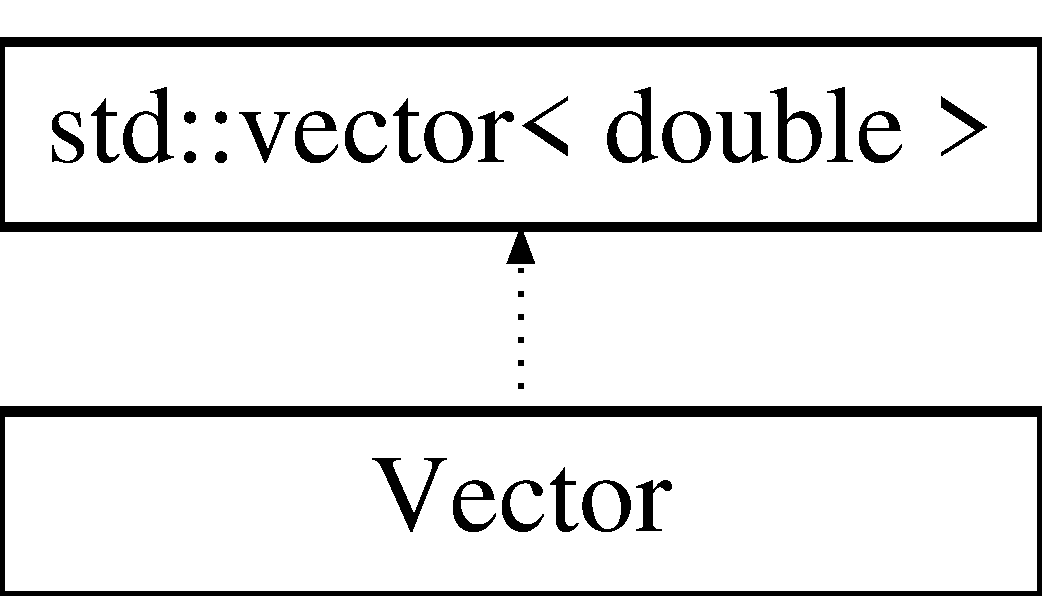
\includegraphics[height=2.000000cm]{class_vector}
\end{center}
\end{figure}
\subsection*{Public Member Functions}
\begin{DoxyCompactItemize}
\item 
\hyperlink{class_vector_a6f80c73b5f18dcf3f8e36065bdc8b9e5}{Vector} ()
\item 
\hyperlink{class_vector_acbdf66550f2caa0a64e0b356fb63a277}{Vector} (int Num)
\item 
\hyperlink{class_vector_a5f04e343b7306ad11f8a82c89b486764}{Vector} (const \hyperlink{class_vector}{Vector} \&v)
\item 
\hyperlink{class_vector}{Vector} \& \hyperlink{class_vector_ae48c467a9f65d60e2f7455aba4ca1239}{operator=} (const \hyperlink{class_vector}{Vector} \&v)
\item 
bool \hyperlink{class_vector_ade5fbd0cd01b034d1907e0c93433320c}{operator==} (const \hyperlink{class_vector}{Vector} \&v) const
\item 
int \hyperlink{class_vector_afbb7966ec4107c43ec15cccc47fcaef7}{get\+Size} () const
\item 
double \hyperlink{class_vector_a6752a90058ddef427ca6aed12946a737}{one\+\_\+norm} () const
\item 
double \hyperlink{class_vector_a4f501290a50d057bb6c57ea64d7e70a4}{two\+\_\+norm} () const
\item 
double \hyperlink{class_vector_a50b72131eaf3698a9876d99ab6912a32}{uniform\+\_\+norm} () const
\end{DoxyCompactItemize}
\subsection*{Friends}
\begin{DoxyCompactItemize}
\item 
std\+::istream \& \hyperlink{class_vector_ac198cff0f4196c66649278458eebf227}{operator$>$$>$} (std\+::istream \&is, \hyperlink{class_vector}{Vector} \&v)
\item 
std\+::ostream \& \hyperlink{class_vector_ac254b27efeb8486ee2f67821e3a21a60}{operator$<$$<$} (std\+::ostream \&os, const \hyperlink{class_vector}{Vector} \&v)
\item 
std\+::ifstream \& \hyperlink{class_vector_ab6009b37fac65598b3db164dc4f19fed}{operator$>$$>$} (std\+::ifstream \&ifs, \hyperlink{class_vector}{Vector} \&v)
\item 
std\+::ofstream \& \hyperlink{class_vector_a8e755f5550c983df730602890058d990}{operator$<$$<$} (std\+::ofstream \&ofs, const \hyperlink{class_vector}{Vector} \&v)
\end{DoxyCompactItemize}


\subsection{Detailed Description}
A vector class for data storage of a 1D array of doubles ~\newline
 The implementation is derived from the standard container vector std\+::vector ~\newline
 We use private inheritance to base our vector upon the library version whilst  usto expose only those base class functions we wish to use -\/ in this  the array access operator \mbox{[}\mbox{]}

The \hyperlink{class_vector}{Vector} class provides\+: ~\newline
-\/basic constructors for creating vector obcjet from other vector object, or by creating empty vector of a given size, ~\newline
-\/input and oput operation via $>$$>$ and $<$$<$ operators using keyboard or file ~\newline
-\/basic operations like access via \mbox{[}\mbox{]} operator, assignment and comparision 

\subsection{Constructor \& Destructor Documentation}
\mbox{\Hypertarget{class_vector_a6f80c73b5f18dcf3f8e36065bdc8b9e5}\label{class_vector_a6f80c73b5f18dcf3f8e36065bdc8b9e5}} 
\index{Vector@{Vector}!Vector@{Vector}}
\index{Vector@{Vector}!Vector@{Vector}}
\subsubsection{\texorpdfstring{Vector()}{Vector()}\hspace{0.1cm}{\footnotesize\ttfamily [1/3]}}
{\footnotesize\ttfamily Vector\+::\+Vector (\begin{DoxyParamCaption}{ }\end{DoxyParamCaption})}

Default constructor. Intialize an empty \hyperlink{class_vector}{Vector} object \begin{DoxySeeAlso}{See also}
\hyperlink{class_vector_acbdf66550f2caa0a64e0b356fb63a277}{Vector(int Num)} 

\hyperlink{class_vector_a5f04e343b7306ad11f8a82c89b486764}{Vector(const Vector\& v)} 
\end{DoxySeeAlso}
\mbox{\Hypertarget{class_vector_acbdf66550f2caa0a64e0b356fb63a277}\label{class_vector_acbdf66550f2caa0a64e0b356fb63a277}} 
\index{Vector@{Vector}!Vector@{Vector}}
\index{Vector@{Vector}!Vector@{Vector}}
\subsubsection{\texorpdfstring{Vector()}{Vector()}\hspace{0.1cm}{\footnotesize\ttfamily [2/3]}}
{\footnotesize\ttfamily Vector\+::\+Vector (\begin{DoxyParamCaption}\item[{int}]{Num }\end{DoxyParamCaption})\hspace{0.3cm}{\ttfamily [explicit]}}

Explicit alterative constructor takes an intiger. it is explicit since implicit type conversion int -\/$>$ vector doesn\textquotesingle{}t make sense Intialize \hyperlink{class_vector}{Vector} object of size Num \begin{DoxySeeAlso}{See also}
\hyperlink{class_vector_a6f80c73b5f18dcf3f8e36065bdc8b9e5}{Vector()} 

\hyperlink{class_vector_a5f04e343b7306ad11f8a82c89b486764}{Vector(const Vector\& v)} 
\end{DoxySeeAlso}

\begin{DoxyExceptions}{Exceptions}
{\em invalid\+\_\+argument} & (\char`\"{}vector size negative\char`\"{}) \\
\hline
\end{DoxyExceptions}

\begin{DoxyParams}{Parameters}
{\em Num} & int. Size of a vector \\
\hline
\end{DoxyParams}
\mbox{\Hypertarget{class_vector_a5f04e343b7306ad11f8a82c89b486764}\label{class_vector_a5f04e343b7306ad11f8a82c89b486764}} 
\index{Vector@{Vector}!Vector@{Vector}}
\index{Vector@{Vector}!Vector@{Vector}}
\subsubsection{\texorpdfstring{Vector()}{Vector()}\hspace{0.1cm}{\footnotesize\ttfamily [3/3]}}
{\footnotesize\ttfamily Vector\+::\+Vector (\begin{DoxyParamCaption}\item[{const \hyperlink{class_vector}{Vector} \&}]{v }\end{DoxyParamCaption})}

Copy constructor takes an \hyperlink{class_vector}{Vector} object reference. Intialize \hyperlink{class_vector}{Vector} object with another \hyperlink{class_vector}{Vector} object \begin{DoxySeeAlso}{See also}
\hyperlink{class_vector_a6f80c73b5f18dcf3f8e36065bdc8b9e5}{Vector()} 

\hyperlink{class_vector_acbdf66550f2caa0a64e0b356fb63a277}{Vector(int Num)} 
\end{DoxySeeAlso}


\subsection{Member Function Documentation}
\mbox{\Hypertarget{class_vector_afbb7966ec4107c43ec15cccc47fcaef7}\label{class_vector_afbb7966ec4107c43ec15cccc47fcaef7}} 
\index{Vector@{Vector}!get\+Size@{get\+Size}}
\index{get\+Size@{get\+Size}!Vector@{Vector}}
\subsubsection{\texorpdfstring{get\+Size()}{getSize()}}
{\footnotesize\ttfamily int Vector\+::get\+Size (\begin{DoxyParamCaption}{ }\end{DoxyParamCaption}) const}

Normal get method that returns integer, the size of the vector \begin{DoxyReturn}{Returns}
int. the size of the vector 
\end{DoxyReturn}
\mbox{\Hypertarget{class_vector_a6752a90058ddef427ca6aed12946a737}\label{class_vector_a6752a90058ddef427ca6aed12946a737}} 
\index{Vector@{Vector}!one\+\_\+norm@{one\+\_\+norm}}
\index{one\+\_\+norm@{one\+\_\+norm}!Vector@{Vector}}
\subsubsection{\texorpdfstring{one\+\_\+norm()}{one\_norm()}}
{\footnotesize\ttfamily double Vector\+::one\+\_\+norm (\begin{DoxyParamCaption}{ }\end{DoxyParamCaption}) const}

Normal public method that returns a double. It returns L1 norm of vector \begin{DoxySeeAlso}{See also}
\hyperlink{class_vector_a4f501290a50d057bb6c57ea64d7e70a4}{two\+\_\+norm()const} 

\hyperlink{class_vector_a50b72131eaf3698a9876d99ab6912a32}{uniform\+\_\+norm()const} 
\end{DoxySeeAlso}
\begin{DoxyReturn}{Returns}
double. vectors L1 norm 
\end{DoxyReturn}
\mbox{\Hypertarget{class_vector_ae48c467a9f65d60e2f7455aba4ca1239}\label{class_vector_ae48c467a9f65d60e2f7455aba4ca1239}} 
\index{Vector@{Vector}!operator=@{operator=}}
\index{operator=@{operator=}!Vector@{Vector}}
\subsubsection{\texorpdfstring{operator=()}{operator=()}}
{\footnotesize\ttfamily \hyperlink{class_vector}{Vector} \& Vector\+::operator= (\begin{DoxyParamCaption}\item[{const \hyperlink{class_vector}{Vector} \&}]{v }\end{DoxyParamCaption})}

Overloaded assignment operator \begin{DoxySeeAlso}{See also}
\hyperlink{class_vector_ade5fbd0cd01b034d1907e0c93433320c}{operator==(const Vector\& v)const} 
\end{DoxySeeAlso}

\begin{DoxyParams}{Parameters}
{\em v} & \hyperlink{class_vector}{Vector} to assign from \\
\hline
\end{DoxyParams}
\begin{DoxyReturn}{Returns}
the object on the left of the assignment 
\end{DoxyReturn}

\begin{DoxyParams}{Parameters}
{\em v} & Vecto\&. \hyperlink{class_vector}{Vector} to assign from \\
\hline
\end{DoxyParams}
\mbox{\Hypertarget{class_vector_ade5fbd0cd01b034d1907e0c93433320c}\label{class_vector_ade5fbd0cd01b034d1907e0c93433320c}} 
\index{Vector@{Vector}!operator==@{operator==}}
\index{operator==@{operator==}!Vector@{Vector}}
\subsubsection{\texorpdfstring{operator==()}{operator==()}}
{\footnotesize\ttfamily bool Vector\+::operator== (\begin{DoxyParamCaption}\item[{const \hyperlink{class_vector}{Vector} \&}]{v }\end{DoxyParamCaption}) const}

Overloaded comparison operator returns true if vectors are the same within a tolerance (1.\+e-\/07) \begin{DoxySeeAlso}{See also}
\hyperlink{class_vector_ae48c467a9f65d60e2f7455aba4ca1239}{operator=(const Vector\& v)} 

operator\mbox{[}$\,$\mbox{]}(int i) 

operator\mbox{[}$\,$\mbox{]}(int i)const 
\end{DoxySeeAlso}
\begin{DoxyReturn}{Returns}
bool. true or false 
\end{DoxyReturn}

\begin{DoxyExceptions}{Exceptions}
{\em invalid\+\_\+argument} & (\char`\"{}incompatible vector sizes\textbackslash{}n\char`\"{}) \\
\hline
\end{DoxyExceptions}

\begin{DoxyParams}{Parameters}
{\em v} & \hyperlink{class_vector}{Vector}\&. vector to compare \\
\hline
\end{DoxyParams}
\mbox{\Hypertarget{class_vector_a4f501290a50d057bb6c57ea64d7e70a4}\label{class_vector_a4f501290a50d057bb6c57ea64d7e70a4}} 
\index{Vector@{Vector}!two\+\_\+norm@{two\+\_\+norm}}
\index{two\+\_\+norm@{two\+\_\+norm}!Vector@{Vector}}
\subsubsection{\texorpdfstring{two\+\_\+norm()}{two\_norm()}}
{\footnotesize\ttfamily double Vector\+::two\+\_\+norm (\begin{DoxyParamCaption}{ }\end{DoxyParamCaption}) const}

Normal public method that returns a double. It returns L2 norm of vector \begin{DoxySeeAlso}{See also}
\hyperlink{class_vector_a6752a90058ddef427ca6aed12946a737}{one\+\_\+norm()const} 

\hyperlink{class_vector_a50b72131eaf3698a9876d99ab6912a32}{uniform\+\_\+norm()const} 
\end{DoxySeeAlso}
\begin{DoxyReturn}{Returns}
double. vectors L2 norm 
\end{DoxyReturn}
\mbox{\Hypertarget{class_vector_a50b72131eaf3698a9876d99ab6912a32}\label{class_vector_a50b72131eaf3698a9876d99ab6912a32}} 
\index{Vector@{Vector}!uniform\+\_\+norm@{uniform\+\_\+norm}}
\index{uniform\+\_\+norm@{uniform\+\_\+norm}!Vector@{Vector}}
\subsubsection{\texorpdfstring{uniform\+\_\+norm()}{uniform\_norm()}}
{\footnotesize\ttfamily double Vector\+::uniform\+\_\+norm (\begin{DoxyParamCaption}{ }\end{DoxyParamCaption}) const}

Normal public method that returns a double. It returns L\+\_\+max norm of vector \begin{DoxySeeAlso}{See also}
\hyperlink{class_vector_a6752a90058ddef427ca6aed12946a737}{one\+\_\+norm()const} 

\hyperlink{class_vector_a4f501290a50d057bb6c57ea64d7e70a4}{two\+\_\+norm()const} 
\end{DoxySeeAlso}

\begin{DoxyExceptions}{Exceptions}
{\em out\+\_\+of\+\_\+range} & (\char`\"{}vector access error\char`\"{}) vector has zero size \\
\hline
\end{DoxyExceptions}
\begin{DoxyReturn}{Returns}
double. vectors Lmax norm 
\end{DoxyReturn}


\subsection{Friends And Related Function Documentation}
\mbox{\Hypertarget{class_vector_ac254b27efeb8486ee2f67821e3a21a60}\label{class_vector_ac254b27efeb8486ee2f67821e3a21a60}} 
\index{Vector@{Vector}!operator$<$$<$@{operator$<$$<$}}
\index{operator$<$$<$@{operator$<$$<$}!Vector@{Vector}}
\subsubsection{\texorpdfstring{operator$<$$<$}{operator<<}\hspace{0.1cm}{\footnotesize\ttfamily [1/2]}}
{\footnotesize\ttfamily std\+::ostream\& operator$<$$<$ (\begin{DoxyParamCaption}\item[{std\+::ostream \&}]{os,  }\item[{const \hyperlink{class_vector}{Vector} \&}]{v }\end{DoxyParamCaption})\hspace{0.3cm}{\ttfamily [friend]}}

Overloaded ifstream $<$$<$ operator. Display output. \begin{DoxySeeAlso}{See also}
\hyperlink{class_vector_ac198cff0f4196c66649278458eebf227}{operator$>$$>$(std\+::istream\& is, Vector\& v)} 

\hyperlink{class_vector_ab6009b37fac65598b3db164dc4f19fed}{operator$>$$>$(std\+::ifstream\& ifs, Vector\& v)} 

\hyperlink{class_vector_a8e755f5550c983df730602890058d990}{operator$<$$<$(std\+::ofstream\& ofs, const Vector\& v)} 
\end{DoxySeeAlso}
\begin{DoxyReturn}{Returns}
std\+::ostream\&. the output stream object os 
\end{DoxyReturn}

\begin{DoxyParams}{Parameters}
{\em os} & output file stream \\
\hline
{\em v} & vector to read from \\
\hline
\end{DoxyParams}
\mbox{\Hypertarget{class_vector_a8e755f5550c983df730602890058d990}\label{class_vector_a8e755f5550c983df730602890058d990}} 
\index{Vector@{Vector}!operator$<$$<$@{operator$<$$<$}}
\index{operator$<$$<$@{operator$<$$<$}!Vector@{Vector}}
\subsubsection{\texorpdfstring{operator$<$$<$}{operator<<}\hspace{0.1cm}{\footnotesize\ttfamily [2/2]}}
{\footnotesize\ttfamily std\+::ofstream\& operator$<$$<$ (\begin{DoxyParamCaption}\item[{std\+::ofstream \&}]{ofs,  }\item[{const \hyperlink{class_vector}{Vector} \&}]{v }\end{DoxyParamCaption})\hspace{0.3cm}{\ttfamily [friend]}}

Overloaded ofstream $<$$<$ operator. File output. the file output operator is compatible with file input operator, ie. everything written can be read later. \begin{DoxySeeAlso}{See also}
\hyperlink{class_vector_ac198cff0f4196c66649278458eebf227}{operator$>$$>$(std\+::istream\& is, Vector\& v)} 

\hyperlink{class_vector_ab6009b37fac65598b3db164dc4f19fed}{operator$>$$>$(std\+::ifstream\& ifs, Vector\& v)} 

\hyperlink{class_vector_ac254b27efeb8486ee2f67821e3a21a60}{operator$<$$<$(std\+::ostream\& os, const Vector\& v)} 
\end{DoxySeeAlso}
\begin{DoxyReturn}{Returns}
std\+::ofstream\&. the output ofstream object ofs 
\end{DoxyReturn}

\begin{DoxyParams}{Parameters}
{\em ofs} & outputfile stream. With opened file \\
\hline
{\em v} & \hyperlink{class_vector}{Vector}\&. vector to read from \\
\hline
\end{DoxyParams}
\mbox{\Hypertarget{class_vector_ac198cff0f4196c66649278458eebf227}\label{class_vector_ac198cff0f4196c66649278458eebf227}} 
\index{Vector@{Vector}!operator$>$$>$@{operator$>$$>$}}
\index{operator$>$$>$@{operator$>$$>$}!Vector@{Vector}}
\subsubsection{\texorpdfstring{operator$>$$>$}{operator>>}\hspace{0.1cm}{\footnotesize\ttfamily [1/2]}}
{\footnotesize\ttfamily std\+::istream\& operator$>$$>$ (\begin{DoxyParamCaption}\item[{std\+::istream \&}]{is,  }\item[{\hyperlink{class_vector}{Vector} \&}]{v }\end{DoxyParamCaption})\hspace{0.3cm}{\ttfamily [friend]}}

Overloaded istream $>$$>$ operator. Keyboard input if vector has size user will be asked to input only vector values if vector was not initialized user can choose vector size and input it values \begin{DoxySeeAlso}{See also}
\hyperlink{class_vector_ab6009b37fac65598b3db164dc4f19fed}{operator$>$$>$(std\+::ifstream\& ifs, Vector\& v)} 

\hyperlink{class_vector_ac254b27efeb8486ee2f67821e3a21a60}{operator$<$$<$(std\+::ostream\& os, const Vector\& v)} 

\hyperlink{class_vector_a8e755f5550c983df730602890058d990}{operator$<$$<$(std\+::ofstream\& ofs, const Vector\& v)} 
\end{DoxySeeAlso}
\begin{DoxyReturn}{Returns}
std\+::istream\&. the input stream object is 
\end{DoxyReturn}

\begin{DoxyExceptions}{Exceptions}
{\em std\+::invalid\+\_\+argument} & (\char`\"{}read error -\/ negative vector size\char`\"{}); \\
\hline
\end{DoxyExceptions}

\begin{DoxyParams}{Parameters}
{\em is} & keyboard input straem. For user input \\
\hline
{\em v} & \hyperlink{class_vector}{Vector}\&. vector to write to \\
\hline
\end{DoxyParams}
\mbox{\Hypertarget{class_vector_ab6009b37fac65598b3db164dc4f19fed}\label{class_vector_ab6009b37fac65598b3db164dc4f19fed}} 
\index{Vector@{Vector}!operator$>$$>$@{operator$>$$>$}}
\index{operator$>$$>$@{operator$>$$>$}!Vector@{Vector}}
\subsubsection{\texorpdfstring{operator$>$$>$}{operator>>}\hspace{0.1cm}{\footnotesize\ttfamily [2/2]}}
{\footnotesize\ttfamily std\+::ifstream\& operator$>$$>$ (\begin{DoxyParamCaption}\item[{std\+::ifstream \&}]{ifs,  }\item[{\hyperlink{class_vector}{Vector} \&}]{v }\end{DoxyParamCaption})\hspace{0.3cm}{\ttfamily [friend]}}

Overloaded ifstream $>$$>$ operator. File input the file output operator is compatible with file input operator, ie. everything written can be read later. \begin{DoxySeeAlso}{See also}
\hyperlink{class_vector_ac198cff0f4196c66649278458eebf227}{operator$>$$>$(std\+::istream\& is, Vector\& v)} 

\hyperlink{class_vector_ac254b27efeb8486ee2f67821e3a21a60}{operator$<$$<$(std\+::ostream\& os, const Vector\& v)} 

\hyperlink{class_vector_a8e755f5550c983df730602890058d990}{operator$<$$<$(std\+::ofstream\& ofs, const Vector\& v)} 
\end{DoxySeeAlso}
\begin{DoxyReturn}{Returns}
ifstream\&. the input ifstream object ifs 
\end{DoxyReturn}

\begin{DoxyExceptions}{Exceptions}
{\em std\+::invalid\+\_\+argument} & (\char`\"{}file read error -\/ negative vector size\char`\"{}); \\
\hline
\end{DoxyExceptions}

\begin{DoxyParams}{Parameters}
{\em ifs} & input file straem. With opened matrix file \\
\hline
{\em v} & \hyperlink{class_vector}{Vector}\&. vector to write to \\
\hline
\end{DoxyParams}


The documentation for this class was generated from the following files\+:\begin{DoxyCompactItemize}
\item 
vector.\+h\item 
vector.\+cpp\end{DoxyCompactItemize}

%--- End generated contents ---

% Index
\backmatter
\newpage
\phantomsection
\clearemptydoublepage
\addcontentsline{toc}{chapter}{Index}
\printindex

\end{document}
